\chapter{Hệ Thống Luyện Nghe Tiếng Anh }

\ifpdf
    \graphicspath{{Chapter3/Chapter3Figs/PNG/}{Chapter3/Chapter3Figs/PDF/}{Chapter3/Chapter3Figs/}}
\else
    \graphicspath{{Chapter3/Chapter3Figs/EPS/}{Chapter3/Chapter3Figs/}}
\fi

\section{Đặt vấn đề}

Các tính năng cần thiết để xây dựng cho chương trình:

\quad - Luyện thi nghe IELTS (offline): một tính năng quan trọng của chương trình. Người sử dụng được làm bài thi nghe của bộ đề IELTS theo hai cách : luyện tập và thi thử.

\quad -	Luyện nghe online: đây là tính năng chủ chốt của chương trình. Người dùng sẽ đăng nhập vào hệ thống bằng tài khoản của Moodle, đăng nhập thành công thì người dùng có thể chọn khóa học mà mình muốn, chọn các bộ đề trong khóa học đó để luyện nghe.

\quad - Hệ thống Moodle sẽ làm nhiệm vụ quản lý tài khoản người dùng, quản lý nội dung bài học, lưu trữ các bộ đề. 

\quad -	Chức năng phụ: Xem thống kê kỹ năng: người sử dụng được xem lại điểm số những bài trắc nghiệm đã làm, với những đánh giá về kỹ năng nghe trong bài một cách khách quan nhất. Từ đó có thể rút ra những điểm yếu của bản thân trong việc luyện nghe.

\begin{figure}[!htb] 
\centering
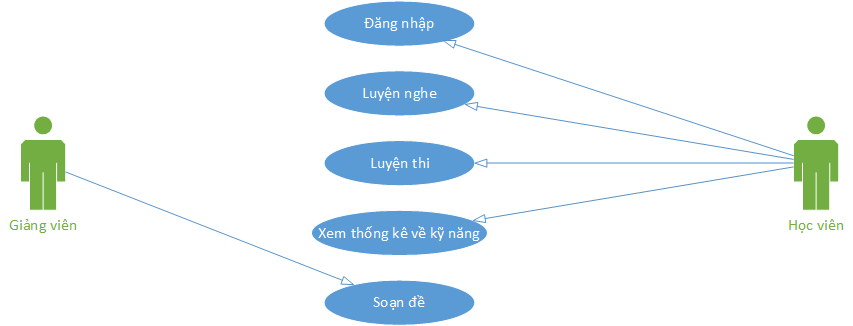
\includegraphics[width=0.8\textwidth]{usecase.png}
\caption{Sơ đồ usecase về các chức năng của ứng dụng}
\end{figure}

\section{Đề thi nghe IELTS}
\subsection{Tại sao lại chọn đề thi IELTS?}

IELTS là một bài kiểm tra về sự thành thạo Anh ngữ, được chấp nhận ở phần lớn các học viện ở Anh, Úc, Canada, Ireland, New Zealand, Nam Phi và ngày càng nhiều các học viện ở Mỹ cũng như nhiều tổ chức nghề nghiệp. Và IELTS đã trở thành hệ thống kiểm tra ngôn ngữ tiếng Anh dành cho bậc sau đại học và người di cư phổ biến nhất trên thế giới. Vì thế bài thi IELTS luôn có một độ khó nhất định và là tiêu chuẩn đánh giá khá chính xác và khách quan về kỹ năng tiếng Anh của người tham dự.

Các câu hỏi và phần audio của chương trình được trích từ các bộ đề thi IELTS phổ thông từ quyển Cambridge IELTS 9.\\
\\
\\
\\
\\
\\
\\
\\
\\
\\
\\
\\
\begin{figure}[!htb] 
\centering
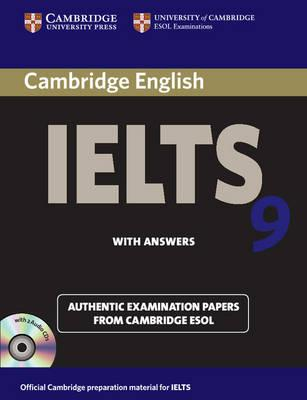
\includegraphics[scale=0.8]{ielts9.png}
\caption{Bìa sách Cambridge IELTS 9 (Nguồn: covers.booktopia.com.au)}
\end{figure}

Vì nội dung chương trình chỉ mang tính chất tham khảo và không vì mục đích lợi nhuận nên nhóm đã sử dụng nội dung trong quyển sách nói trên. Nếu phát triển thành ứng dụng có tính phí, nhóm sẽ thay đổi với những nội dung có bản quyền.

\subsection{Cấu trúc bài thi}

Thời gian làm bài thi nghe là 40 phút với 40 câu hỏi, trong đó 30 phút là thời gian đoạn băng được phát cho bài thi nghe, và sẽ có 10 phút sau đó để thí sinh điền đáp án vào phiếu trả lời. Thí sinh sẽ nghe tất cả các câu hỏi và độ khó của từng câu sẽ tăng dần. Bài thi bao gồm nhiều dạng khác nhau như thông tin từ một người, cuộc đàm thoại của 2 hoặc nhiều người. Và thí sinh sẽ nghe nhiều giọng phát âm của nhiều quốc gia khác nhau. Thí sinh chỉ nghe được 1 lần. Tuy nhiên, bạn sẽ có thời gian để đọc câu hỏi và chuẩn bị câu trả lời. Bài thi nghe có 4 phần (số câu hỏi không được chia đều), nghe 1 lần và các đoạn nghỉ được ghi kèm trong băng hoặc đĩa. Cuối bài thi các thí sinh sẽ có 10 phút để ghi lại kết quả vào Phiếu trả lời câu hỏi.

\quad Phần 1: là các tình huống đời thường (đăng ký hoạt động, thuê nhà, nhập học) thường là 1 cuộc nói chuyện nhưng là hỏi đáp, và người đáp thường nói nhiều hơn.

\quad Phần 2: là các tình huống hướng dẫn và giới thiệu về 1 chủ đề quen thuộc (trường học, khu du lịch, chương trình ca nhạc, triển lãm,..) thường chỉ nói bởi 1 người.

\quad Phần 3: là các tình huống đối thoại giữa ít nhất là 2 người, đây là các cuộc thảo luận có tính chất học thuật hơn (Ví dụ: chọn chủ đề khóa luận, đề tài nghiên cứu khoa học).

\quad Phần 4: là 1 bài thuyết trình về 1 chủ đề học thuật, thường do 1 người nói và dùng nhiều từ ngữ mang tính chất học thuật.

\subsection{Cách tính điểm}

Bài thi Nghe bao gồm 40 câu. 1 câu trả lời đúng thí sinh sẽ được 1 điểm. Số điểm tối đa có thể đạt được là 40 cho từng bài thi. Thang điểm từ 1 – 9 sẽ được tính dựa trên số câu trả lời đúng. Cụ thể như sau:\\

\begin{figure}[htb] 
\centering
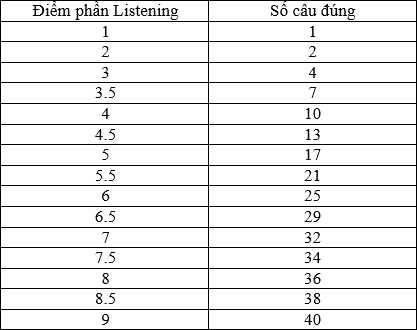
\includegraphics[scale=0.8]{score.png}
\caption{Thang điểm trong phần nghe của đề IELTS}
\end{figure}

\subsection{Các dạng câu hỏi}

Trong phần thi nghe của bài kiểm tra IELTS, thí sinh được nghe những đoạn audio về  3 đoạn hội thoại ở phần 1, 2, 3 và 1 chủ đề ở phần 4. Chủ yếu có các dạng câu hỏi sau:

\quad - Dạng câu hỏi điền từ vào chỗ trống: thí sinh sẽ điền những từ/cụm từ với số lượng chữ/chữ số được cho theo yêu cầu đề bài. Câu trả lời là chính xác nếu từ khóa của thí sinh trùng với từ khóa của đáp án. Trong một câu hỏi có thể có 2 ô trống để điền từ.

\begin{figure}[htb] 
\centering
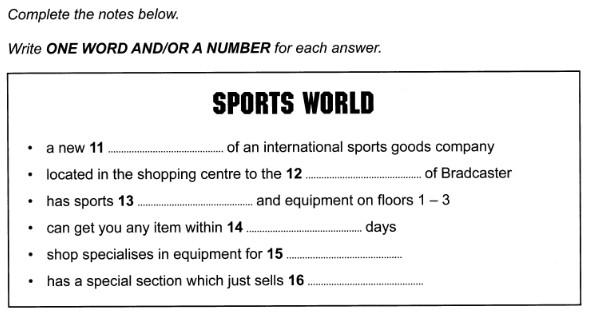
\includegraphics[scale=0.4]{ques_fill.png}
\caption{Mẫu câu hỏi điền từ vào mẩu thông tin}
\end{figure}

\quad - Ở dạng câu hỏi này, có thể có kiểu câu hỏi bắt thí sinh điền vào chỗ trống những phương án đề cho sẵn như TRUE, FALSE hoặc NOT GIVEN hoặc dạng điền thông tin vào sơ đồ, bảng biểu.

\begin{figure}[!htb] 
\centering
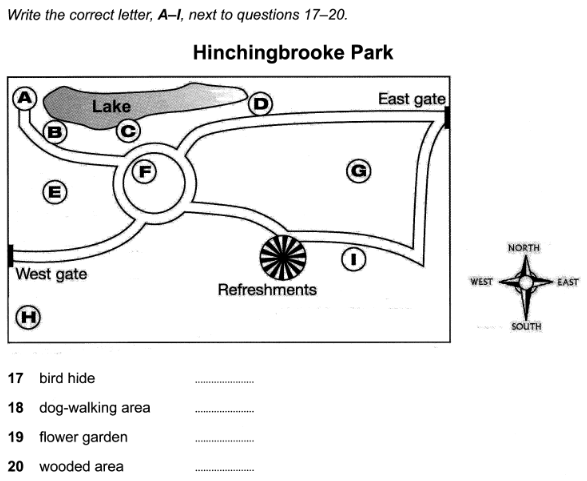
\includegraphics[scale=0.4]{ques_fill2.png}
\caption{Mẫu câu hỏi điền thông tin vào sơ đồ}
\end{figure}

\quad - Dạng câu hỏi trắc nghiệm: thí sinh sẽ nghe đoạn băng và trả lời câu hỏi với 3 phương án A, B, C với 1 lựa chọn thí sinh cho là đúng, hoặc 2 lựa chọn với dạng câu hỏi có 5 phương án A, B, C, D, E.

\begin{figure}[!htb] 
\centering
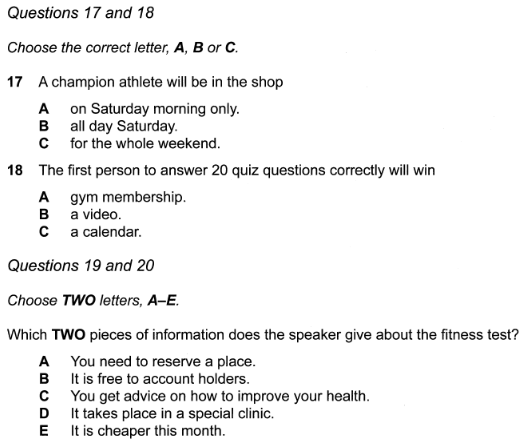
\includegraphics[scale=0.4]{ques_multi.png}
\caption{Mẫu câu hỏi trắc nghiệm}
\end{figure}

\subsection{Số hóa câu hỏi bằng các thành phần XML}

Dữ liệu của câu hỏi và các thông tin đi kèm, các phương án trả lời sẽ được lưu thành một file XML có cấu trúc đơn giản và được truyền về máy khách khi có yêu cầu. Sau đó, file XML sẽ được duyệt và hiển thị lên màn hình các thông tin được lưu trong file. Cấu trúc file XML như sau:

\begin{figure}[!htb] 
\centering
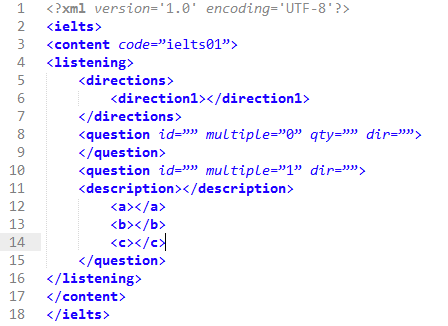
\includegraphics[scale=0.8]{xml.png}
\caption{Cấu trúc XML lưu trữ câu hỏi}
\end{figure}

Trong đó, chức năng của các thẻ như sau:

\quad - Thẻ <ielts> là thẻ root của file XML

\quad - Thẻ <content> có tham số code=”ielts01” chính là mã đề của đề hiện tại.

\quad - Thẻ <directions> chứa các chỉ dẫn làm bài của các câu hỏi, về loại câu hỏi và các thông tin cần thiết giúp thí sinh làm bài tốt hơn. Nhiều câu hỏi có thể có phần chỉ dẫn giống nhau.

\quad - Thẻ <question> chứa các thông tin về câu hỏi. Có 2 loại:

\quad \quad + Loại có tham số multiple=”0” là các dạng câu hỏi điền từ, với phần nội dung của thẻ là đoạn mã HTML đã được định dạng và được gói trong cú pháp CDATA. Những ô trống để thí sinh có thể điền từ vào được thể hiện trong mã HTML bằng thẻ <div id=”” class=” questext”></div>.

\quad \quad + Loại có tham số multiple=”1” là các dạng câu hỏi trắc nghiệm. Thẻ này có các thẻ con như <description> chứa thông tin câu hỏi và các thẻ <a>, <b>, <c> chứa các phương án lựa chọn trả lời. Đặc biệt là loại có tham số multiple=”2” là câu hỏi trắc nghiệm có 5 phương án lựa chọn với các thẻ phương án là <a>, <b>, <c>, <d> và <e>. Trong đó, thí sinh được chọn 2 phương án trả lời được cho là đúng.





\section{Thiết kế các tính năng ứng dụng}
Chương trình sẽ được phát triển theo mô hình truyền thông giữa Client và Server, trong đó, Moodle sẽ đóng vai trò làm Server, còn các tablet của người sử dụng là Client. Việc kết nối sẽ được thực hiện qua giao thức TCP/IP.
\newpage
\begin{figure}[!htb] 
\centering
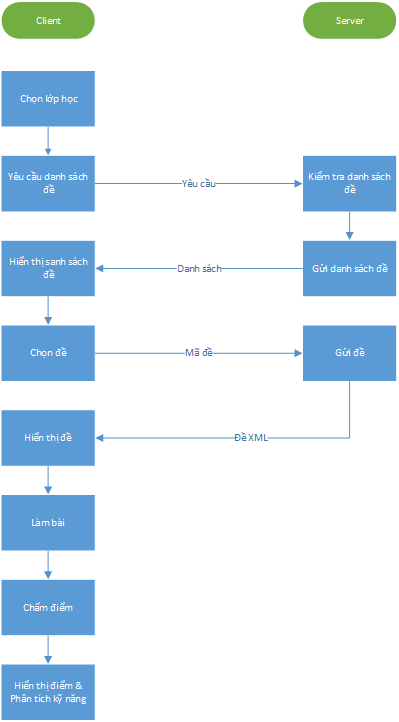
\includegraphics[width=0.6\textwidth]{flowchart.png}
\caption{Sơ đồ luồng chung của ứng dụng}
\end{figure}


\subsection{Thiết kế tính năng luyện nghe Offline}
Client sẽ kiểm tra danh sách đề thi trong dữ liệu chương trình. Sau đó sẽ hiển thị danh sách các đề hiện có.

Người sử dụng sẽ chọn đề. Nội dung đề được trả về là file XML và file audio.

Nội dung audio sẽ được phát, đồng thời client hiển thị nội dung câu hỏi cho người sử dụng làm bài.

\begin{figure}[!htb] 
\centering
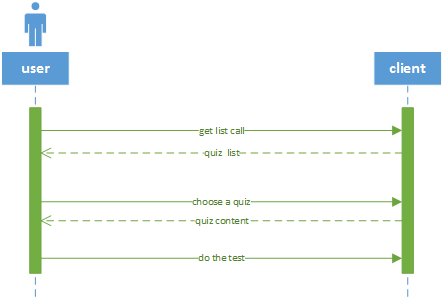
\includegraphics[width=0.8\textwidth]{getQuesSeq.png}
\caption{Sơ đồ sequence về hoạt động tải đề kiểm tra khi chạy offline}
\end{figure}

\subsection{Thiết kế tính năng đăng nhập và lấy token}

Khi bắt chương trình, giữa client và server sẽ thiết lập một kết nối truyền tải dữ liệu.

Sau khi người sử dụng nhập các thông tin tài khoản như tên tài khoản và mật khẩu, dữ liệu sẽ được gửi đến server.

Server sẽ kiểm tra thông tin và gửi trả về token xác thực phiên sử dụng của tài khoản nếu tên tài khoản và mật khẩu được gửi đến là đúng.

Kể từ đó, mỗi lời gọi đến server của client đều phải đính kèm token xác thực. Và server gửi trả thông tin được yêu cầu tương ứng.\\
\\
\\
\\
\begin{figure}[!htb] 
\centering
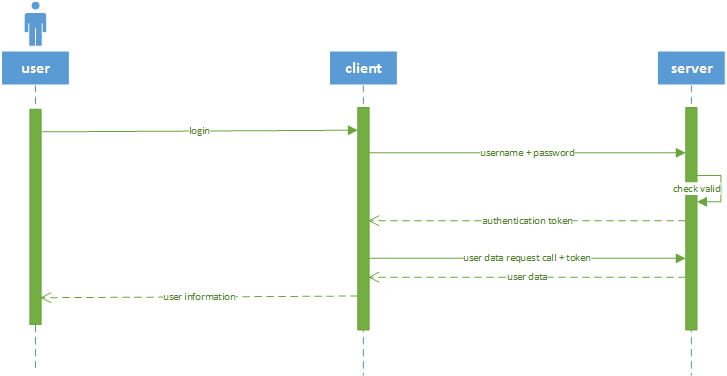
\includegraphics[width=0.8\textwidth]{loginSequence.png}
\caption{Sơ đồ sequence về hoạt động đăng nhập}
\end{figure}
\\

\subsection{Thiết kế tính năng lấy đề luyện nghe}

Sau khi đăng nhập thành công, client sẽ gửi yêu cầu danh sách đề thi kèm theo token cho server. Server sẽ gửi trả danh sách các đề đang có.

Người sử dụng sẽ chọn đề theo 3 mức độ khó. Id của đề sẽ được gửi lại cho server và server trả về nội dung đề là file XML và file audio.

Nội dung audio sẽ được phát, đồng thời client hiển thị nội dung câu hỏi cho người sử dụng làm bài.

\begin{figure}[!htb] 
\centering
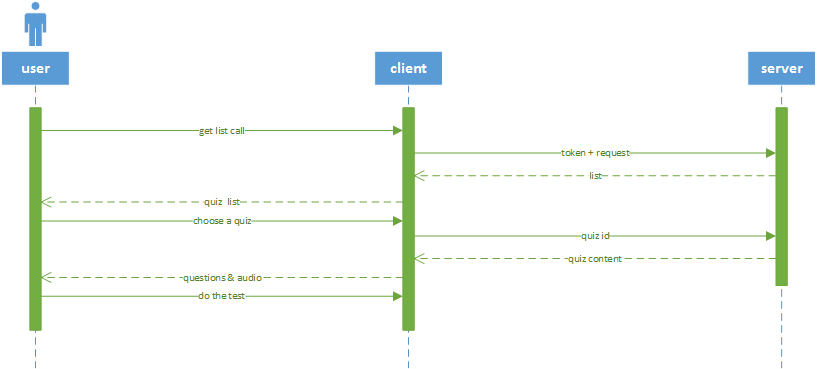
\includegraphics[width=0.8\textwidth]{getQuizSequence.png}
\caption{Sơ đồ sequence về hoạt động tải đề kiểm tra}
\end{figure}
\newpage

\subsection{Thiết kế tính năng chấm bài và đánh giá kỹ năng}

Sau khi người sử dụng làm bài xong và nhấn Submit, danh sách câu trả lời được gửi đến server.

Server sẽ dò và so sánh danh sách câu trả lời vừa nhận với danh sách đáp án đã lưu trước dựa theo mã đề. Câu trả lời đúng là câu trả lời có nội dung trùng với từ khóa trong đáp án.

Sau khi chấm, danh sách số câu trả lời đúng theo từng Section sẽ được gửi về cho client. Từ đó, client đánh giá được kỹ năng của người dùng dựa trên số điểm của mỗi Section với mỗi kỹ năng riêng.

\begin{figure}[!htb] 
\centering
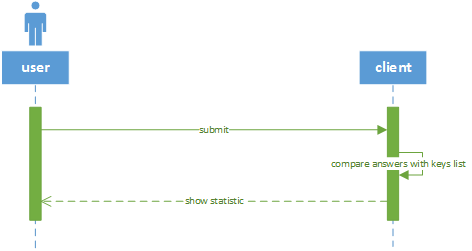
\includegraphics[width=0.8\textwidth]{getMarkSequenceOff.png}
\caption{Sơ đồ sequence về hoạt động nộp bài và chấm bài}
\end{figure}
\newpage

\section{Tổng kết chương}

Trong chương này, nhóm chúng em đã trình bày về đặc điểm của các câu hỏi trong bộ đề thi nghe IELTS để biểu diễn chúng dưới dạng dữ liệu và tìm ra cách thức tiếp cận, giải quyết các luồng hoạt động của chương trình.

Tuy nhiên, ở chương này, các bản thiết kế chỉ ở mức sơ bộ. Chúng em sẽ hoàn thiện các sơ đồ thiết kế này thành một ứng dụng hoàn chỉnh ở chương sau.
